\documentclass{assignment}
\usepackage{amsmath}
\usepackage{graphicx}
\usepackage{paracol}
\begin{document}
\title{Assignment 1}
\author{NYALAPOGULA MANASWINI(CS20btech11035)}
\maketitle
\begin{paracol}{2}
\switchcolumn[0]
\begin{Large}
QUESTION:\\
Suppose X has a binomial distribution . Show
that X = 3 is the most likely outcome.
(Hint : P(X = 3) is the maximum among all
P($x_i$), $x_i$= 0,1,2,3,4,5,6).Assume p=0.5\\
\\
SOLUTION:\\
Given number of times event is performed(n)=6\\
Given probability of event(p)=0.5\\
Therefore 1-p=0.5\\
We know that binomial probability[P(X=k)]=$\binom{n}{k}p^k({1-p})^{n-k}$\\
substituting n=6,p=1-p=$\frac{1}{2}$\\
\begin{align*}
P(X=k)=\binom{6}{k}(\frac{1}{2})^k(\frac{1}{2})^{6-k}\\
(\frac{1}{2})^k(\frac{1}{2})^{6-k}=\frac{1}{2})^{6-k+k}=(\frac{1}{2})^6\\
P(X=k)=\binom{6}{k}(\frac{1}{2})^6
\end{align*}

For P(X=k) to be maximum $\binom{6}{k}$should be maximum ,where k=\{0,1,2,3,4,5,6\}
$\binom{6}{0}=1  , \binom{6}{1}=6,\binom{6}{2}=15,\binom{6}{3}=20,\binom{6}{4}=15,\binom{6}{5}=6,\binom{6}{6}=1$\\
Therefore $\binom{6}{3}$ is maximum ,therefore P(X=3) is most likely outcome.\\
Hence proved.
\switchcolumn[1]
\begin{figure}
\begin{center}
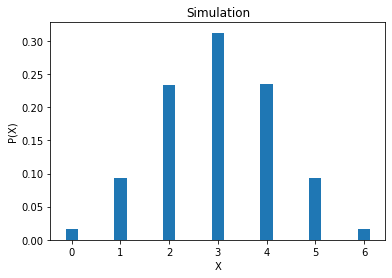
\includegraphics[width=0.58\textwidth]{assignment1.png}
\end{center}
\end{figure}
\end{Large}
\end{paracol}

\end{document}